% answers.tex —— 2008 年·普通高等学校招生考试·重庆卷·文科 · 参考答案与详细解析片段
% 由 tools/generate_projects.py 依来源总账自 2008/2008_数学真题_重庆文_试题.md + 2008/2008_数学真题_重庆文_解析正文.md + 2008/2008_数学真题_重庆文_答案要点.md 生成，勿手改（改源 MD 后重跑）


\begin{gktip}
固定候选 PDF 仅含题面、无答案与解析；以下为非官方编者独立推导。
\end{gktip}

\begin{answer}
\gksolhead{1}{}

\textbf{题目}：

已知 $\{a_n\}$ 为等差数列，$a_2+a_8=12$，则 $a_5$ 等于（　）

（A）$4$

（B）$5$

（C）$6$

（D）$7$

\Needspace{4\baselineskip}
\textbf{解析}

$a_2+a_8=2a_5=12$，故 $a_5=6$。

\gkanswer{答案：C。}

\end{answer}
\begin{answer}
\gksolhead{2}{}

\textbf{题目}：

设 $x$ 是实数，则“$x>0$”是“$|x|>0$”的（　）

（A）充分而不必要条件

（B）必要而不充分条件

（C）充要条件

（D）既不充分也不必要条件

\Needspace{4\baselineskip}
\textbf{解析}

$x>0\Rightarrow|x|>0$；反之 $|x|>0$ 只说明 $x\neq0$，故为充分不必要。

\gkanswer{答案：A。}

\end{answer}
\begin{answer}
\gksolhead{3}{}

\textbf{题目}：

曲线 $C:\begin{cases}x=\cos\theta-1,\\ y=\sin\theta+1,\end{cases}$（$\theta$ 为参数）的普通方程为（　）

（A）$(x-1)^2+(y+1)^2=1$

（B）$(x+1)^2+(y+1)^2=1$

（C）$(x+1)^2+(y-1)^2=1$

（D）$(x-1)^2+(y-1)^2=1$

\Needspace{4\baselineskip}
\textbf{解析}

$x+1=\cos\theta$，$y-1=\sin\theta$，故 $(x+1)^2+(y-1)^2=1$。

\gkanswer{答案：C。}

\end{answer}
\begin{answer}
\gksolhead{4}{}

\textbf{题目}：

若点 $P$ 分有向线段 $\overrightarrow{AB}$ 所成的比为 $-\dfrac13$，则点 $B$ 分有向线段 $\overrightarrow{PA}$ 所成的比是（　）

（A）$-\dfrac32$

（B）$-\dfrac12$

（C）$\dfrac12$

（D）$3$

\Needspace{4\baselineskip}
\textbf{解析}

设 $A=0$，$B=1$，$P=p$，由 $\dfrac{p}{1-p}=-\dfrac13$ 得 $p=-\dfrac12$。此时 $B$ 分 $\overrightarrow{PA}$ 的比为 $\dfrac{1-\left(-\frac12\right)}{0-1}=-\dfrac32$。

\gkanswer{答案：A。}

\end{answer}
\begin{answer}
\gksolhead{5}{}

\textbf{题目}：

某交高三年级有男生 $500$ 人，女生 $400$ 人。为了解该年级学生的健康情况，从男生中任意抽取 $25$ 人，从女生中任意抽取 $20$ 人进行调查。这种抽样方法是（　）

（A）简单随机抽样法

（B）抽签法

（C）随机数表法

（D）分层抽样法

\Needspace{4\baselineskip}
\textbf{解析}

按男、女分层并按比例抽取，为分层抽样法。

\gkanswer{答案：D。}

\end{answer}
\begin{answer}
\gksolhead{6}{}

\textbf{题目}：

函数 $y=10^{x^2-1}$（$0<x\leqslant1$）的反函数是（　）

（A）$y=-\sqrt{1+\lg x}$（$x>\dfrac1{10}$）

（B）$y=\sqrt{1+\lg x}$（$x>\dfrac1{10}$）

（C）$y=-\sqrt{1+\lg x}$（$\dfrac1{10}<x\leqslant1$）

（D）$y=\sqrt{1+\lg x}$（$\dfrac1{10}<x\leqslant1$）

\Needspace{4\baselineskip}
\textbf{解析}

$0<x\leqslant1$ 时 $x^2-1\in\left(-1,0\right]$，$y\in\left(\dfrac1{10},1\right]$；由 $y=10^{x^2-1}$ 得 $x=\sqrt{1+\lg y}$（取正），交换 $x$、$y$ 即得。

\gkanswer{答案：D。}

\end{answer}
\begin{answer}
\gksolhead{7}{}

\textbf{题目}：

函数 $f(x)=\dfrac{\sqrt x}{x+1}$ 的最大值为（　）

（A）$\dfrac25$

（B）$\dfrac12$

（C）$\dfrac{\sqrt2}2$

（D）$1$

\Needspace{4\baselineskip}
\textbf{解析}

$f'(x)=\dfrac{(x+1)-2x}{2\sqrt x(x+1)^2}=\dfrac{1-x}{2\sqrt x(x+1)^2}$，故 $x=1$ 处取最大值 $\dfrac12$。

\gkanswer{答案：B。}

\end{answer}
\begin{answer}
\gksolhead{8}{}

\textbf{题目}：

若双曲线 $\dfrac{x^2}3-\dfrac{16y^2}{p^2}=1$ 的左焦点在抛物线 $y^2=2px$ 的准线上，则 $p$ 的值为（　）

（A）$2$

（B）$3$

（C）$4$

（D）$4\sqrt2$

\Needspace{4\baselineskip}
\textbf{解析}

双曲线 $c^2=3+\dfrac{p^2}{16}$，左焦点 $\left(-c,0\right)$ 在 $x=-\dfrac p2$ 上，故 $c=\dfrac p2$，得 $3+\dfrac{p^2}{16}=\dfrac{p^2}4$，$p^2=16$，$p=4$。

\gkanswer{答案：C。}

\end{answer}
\begin{answer}
\gksolhead{9}{}

\textbf{题目}：

从编号为 $1$，$2$，$\cdots$，$10$ 的 $10$ 个大小相同的球中任取 $4$ 个，则所取 $4$ 个球的最大号码是 $6$ 的概率为（　）

（A）$\dfrac1{84}$

（B）$\dfrac1{21}$

（C）$\dfrac25$

（D）$\dfrac35$

\Needspace{4\baselineskip}
\textbf{解析}

最大号码为 $6$ 即 $6$ 必取、其余三个从 $1\sim5$ 中取：$\dfrac{\mathrm C_5^3}{\mathrm C_{10}^4}=\dfrac{10}{210}=\dfrac1{21}$。

\gkanswer{答案：B。}

\end{answer}
\begin{answer}
\gksolhead{10}{}

\textbf{题目}：

若 $\left(x+\dfrac1{2x}\right)^n$ 的展开式中前三项的系数成等差数列，则展开式中 $x^4$ 项的系数为（　）

（A）$6$

（B）$7$

（C）$8$

（D）$9$

\Needspace{4\baselineskip}
\textbf{解析}

前三项系数 $1$、$\dfrac n2$、$\dfrac{n(n-1)}8$ 成等差，得 $n=8$；$x^4$ 项对应 $k=2$，系数 $\dfrac{\mathrm C_8^2}{2^2}=7$。

\gkanswer{答案：B。}

\end{answer}
\begin{answer}
\gksolhead{11}{}

\textbf{题目}：

如图，模块①～⑤均由 $4$ 个棱长为 $1$ 的小正方体构成，模块⑥由 $15$ 个棱长为 $1$ 的小正方体构成。现从模块①～⑤中选出三个放到模块⑥上，使得模块⑥成为一个棱长为 $3$ 的大正方体。则下列选择方案中，能够完成任务的是（　）
\nopagebreak[4]
\begin{center}% 2008 年重庆卷文科第 11 题：模块①～⑤ 各 4 个单位小正方体，模块⑥ 15 个。
% 来源 PDF：gaokaomath-src/普通高考/2008/2008重庆文.pdf
% SHA-256：a3f3321148dc97354de71daf028e7718ef3c3d89e634f94291448acc1f55ce08
% 原页：2008重庆文.pdf 第 1 页（A3 三栏）第 2 栏，书页码 431。
% 绘制依据：逐块判读原图并做隐藏线消除（只画外露面）：
%   ① 三连排 + 右端上叠；② 2×2 平铺；③ 三连排 + 中上叠；④ 三连排 + 端部向里；
%   ⑤ 三连排 + 中上叠且右端再抬升；⑥ 为 3×3×2 缺 3 块（前中上、右前上、右中上），共 15 块。
\makeatletter
\newcommand{\markcell}[3]{\expandafter\gdef\csname cell#1.#2.#3\endcsname{1}}
\newcommand{\ifnocell}[4]{\ifcsname cell#1.#2.#3\endcsname\else#4\fi}
\makeatother
\newcommand{\cube}[3]{%
  \pgfmathsetmacro{\cx}{#1*0.62+#2*0.30}%
  \pgfmathsetmacro{\cy}{#3*0.62+#2*0.18}%
  \ifnocell{#1}{\the\numexpr#2-1\relax}{#3}{%
    \draw[fill=white] (\cx,\cy) rectangle ++(0.62,0.62);}%
  \ifnocell{#1}{#2}{\the\numexpr#3+1\relax}{%
    \draw[fill=white] (\cx,\cy+0.62) -- ++(0.30,0.18) -- ++(0.62,0) -- ++(-0.30,-0.18) -- cycle;}%
  \ifnocell{\the\numexpr#1+1\relax}{#2}{#3}{%
    \draw[fill=white] (\cx+0.62,\cy) -- ++(0.30,0.18) -- ++(0,0.62) -- ++(-0.30,-0.18) -- cycle;}%
}
\newcommand{\drawmodule}[1]{%
  \foreach \c in {#1} { \markcell\c }%
  \foreach \j in {2,1,0} { \foreach \c in {#1} { \expandafter\ifnum\expandafter`\c<0 \else\fi } }%
}
\begin{tikzpicture}[scale=0.60, semithick, font=\scriptsize, every node/.style={inner sep=1pt}]

  % ---- 模块①：三连排 + 右端上叠 ----
  \begin{scope}
    \markcell{0}{0}{0}\markcell{1}{0}{0}\markcell{2}{0}{0}\markcell{2}{0}{1}
    \cube{0}{0}{0}\cube{1}{0}{0}\cube{2}{0}{0}\cube{2}{0}{1}
    \node at (0.93,-0.45) {模块①};
  \end{scope}

  % ---- 模块②：2×2 平铺 ----
  \begin{scope}[shift={(2.9,0)}]
    \markcell{0}{0}{0}\markcell{1}{0}{0}\markcell{0}{1}{0}\markcell{1}{1}{0}
    \cube{0}{1}{0}\cube{1}{1}{0}\cube{0}{0}{0}\cube{1}{0}{0}
    \node at (0.93,-0.45) {模块②};
  \end{scope}

  % ---- 模块③：三连排 + 中上叠 ----
  \begin{scope}[shift={(5.8,0)}]
    \markcell{0}{0}{0}\markcell{1}{0}{0}\markcell{2}{0}{0}\markcell{1}{0}{1}
    \cube{0}{0}{0}\cube{1}{0}{0}\cube{2}{0}{0}\cube{1}{0}{1}
    \node at (0.93,-0.45) {模块③};
  \end{scope}

  % ---- 模块④：三连排 + 端部向里 ----
  \begin{scope}[shift={(8.7,0)}]
    \markcell{0}{0}{0}\markcell{1}{0}{0}\markcell{2}{0}{0}\markcell{2}{1}{0}
    \cube{2}{1}{0}\cube{0}{0}{0}\cube{1}{0}{0}\cube{2}{0}{0}
    \node at (0.93,-0.45) {模块④};
  \end{scope}

  % ---- 模块⑤：三连排 + 中上叠 + 右端抬升 ----
  \begin{scope}[shift={(11.6,0)}]
    \markcell{0}{0}{0}\markcell{1}{0}{0}\markcell{2}{0}{0}\markcell{1}{0}{1}
    \cube{0}{0}{0}\cube{1}{0}{0}\cube{2}{0}{0}\cube{1}{0}{1}
    \node at (0.93,-0.45) {模块⑤};
  \end{scope}

  % ---- 模块⑥：3×3×2 缺 3 块（前中上、右前上、右中上） ----
  \begin{scope}[shift={(14.8,0)}]
    \markcell{0}{0}{0}\markcell{0}{0}{1}\markcell{0}{1}{0}\markcell{0}{1}{1}\markcell{0}{2}{0}\markcell{0}{2}{1}\markcell{1}{0}{0}\markcell{1}{1}{0}\markcell{1}{1}{1}\markcell{1}{2}{0}\markcell{1}{2}{1}\markcell{2}{0}{0}\markcell{2}{1}{0}\markcell{2}{2}{0}\markcell{2}{2}{1}
    \cube{2}{2}{0}\cube{1}{2}{0}\cube{0}{2}{0}\cube{2}{2}{1}\cube{1}{2}{1}\cube{0}{2}{1}\cube{2}{1}{0}\cube{1}{1}{0}\cube{0}{1}{0}\cube{1}{1}{1}\cube{0}{1}{1}\cube{2}{0}{0}\cube{1}{0}{0}\cube{0}{0}{0}\cube{0}{0}{1}
    \node at (1.24,-0.45) {模块⑥};
  \end{scope}
\end{tikzpicture}
\end{center}
\nopagebreak[4]
（A）模块①②⑤

（B）模块①③⑤

（C）模块②④⑥

（D）模块③④⑤

\Needspace{4\baselineskip}
\textbf{解析}

【判读依据：按原页 450\% 放大，模块⑥是 $3\times3\times2$ 的 $18$ 块去掉 $3$ 块（前中上、右前上、右中上），共 $15$ 块；补成 $3\times3\times3$ 还需 $12$ 块，即顶层 $9$ 块加第二层缺口 $3$ 块。三个 $4$ 块模块必须在顶层各铺一条三连排、并向第二层各补一块，只有①③⑤ 都是"三连排 + 上叠一块"，故填法唯一对应 (B)；②、④ 为平铺，只能铺顶层而补不了第二层缺口。】

\gkanswer{答案：B。}

\end{answer}
\begin{answer}
\gksolhead{12}{}

\textbf{题目}：

函数 $f(x)=\dfrac{\sin x}{\sqrt{5+4\cos x}}$（$0\leqslant x\leqslant2\pi$）的值域是（　）

（A）$\left[-\dfrac14,\dfrac14\right]$

（B）$\left[-\dfrac13,\dfrac13\right]$

（C）$\left[-\dfrac12,\dfrac12\right]$

（D）$\left[-\dfrac23,\dfrac23\right]$

\Needspace{4\baselineskip}
\textbf{解析}

令 $t=\cos x\in[-1,1]$，则 $f^2=\dfrac{1-t^2}{5+4t}$，其最大值在 $t=-\dfrac12$ 处为 $\dfrac14$，故 $f$ 的值域为 $\left[-\dfrac12,\dfrac12\right]$。

\gkanswer{答案：C。}

\end{answer}
\begin{answer}
\gksolhead{13}{}

\textbf{题目}：

设集合 $U=\{1,2,3,4,5\}$，$A=\{2,3,4\}$，$B=\{4,5\}$，则 $A\cap(\complement_UB)=$\gkblank{}。

\Needspace{4\baselineskip}
\textbf{解析}

$\complement_UB=\{1,2,3\}$，故 $A\cap(\complement_UB)=\{2,3\}$。

\gkanswer{答案：$\{2,3\}$。}

\end{answer}
\begin{answer}
\gksolhead{14}{}

\textbf{题目}：

若 $x>0$，则 $\left(2x^{\frac14}+3^{\frac32}\right)\left(2x^{\frac14}-3^{\frac32}\right)-4x^{-\frac12}\left(x-x^{\frac12}\right)=$\gkblank{}。

\Needspace{4\baselineskip}
\textbf{解析}

平方差得 $4x^{\frac12}-27$，减去 $4x^{\frac12}-4$，结果为 $-23$。

\gkanswer{答案：$-23$。}

\end{answer}
\begin{answer}
\gksolhead{15}{}

\textbf{题目}：

已知圆 $C:x^2+y^2+2x+ay-3=0$（$a$ 为实数）上任意一点关于直线 $l:x-y+2=0$ 的对称点都在圆 $C$ 上，则 $a=$\gkblank{}。

\Needspace{4\baselineskip}
\textbf{解析}

圆关于直线对称等价于圆心 $\left(-1,-\dfrac a2\right)$ 在 $x-y+2=0$ 上，即 $-1+\dfrac a2+2=0$，$a=-2$。

\gkanswer{答案：$-2$。}

\end{answer}
\begin{answer}
\gksolhead{16}{}

\textbf{题目}：

某人有 $3$ 种颜色的灯泡（每种颜色的灯泡足够多），要在如图所示的 $6$ 个点 $A$、$B$、$C$、$A_1$、$B_1$、$C_1$ 上各装一个灯泡，要求同一条线段两端的灯泡不同色，则不同的安装方法共有\gkblank{}种。（用数字作答）
\nopagebreak[4]
\begin{center}% 2008 年重庆卷文科第 16 题：三棱柱 ABC-A1B1C1 的 6 个顶点上各装一个灯泡，
%   同一条线段两端不同色，3 种颜色可选。
% 来源 PDF：gaokaomath-src/普通高考/2008/2008重庆文.pdf
% SHA-256：a3f3321148dc97354de71daf028e7718ef3c3d89e634f94291448acc1f55ce08
% 原页：2008重庆文.pdf 第 1 页（A3 三栏）第 2 栏，书页码 431。
% 重绘依据：按原页画三棱柱：上底 A、B、C，下底 A1、B1、C1；可见棱 A—B、A—C、B—C、
%   A—A1、B—B1、A1—B1 实线，隐藏棱 C—C1、A1—C1、B1—C1 虚线。
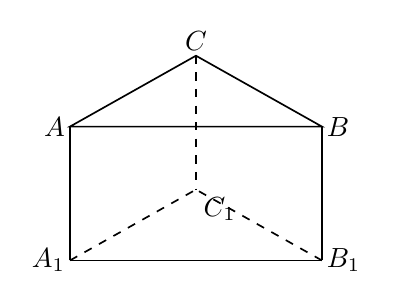
\begin{tikzpicture}[scale=1.0, semithick, every node/.style={inner sep=1.5pt}]
  \coordinate (A) at (-1.60,1.05);
  \coordinate (B) at (1.60,1.05);
  \coordinate (C) at (0.00,1.95);
  \coordinate (A1) at (-1.60,-0.65);
  \coordinate (B1) at (1.60,-0.65);
  \coordinate (C1) at (0.00,0.25);

  \draw (A) -- (B) -- (C) -- cycle;
  \draw (A) -- (A1);
  \draw (B) -- (B1);
  \draw (A1) -- (B1);
  \draw[dashed] (C) -- (C1);
  \draw[dashed] (A1) -- (C1);
  \draw[dashed] (B1) -- (C1);

  \node[left] at (A) {$A$};
  \node[right] at (B) {$B$};
  \node[above] at (C) {$C$};
  \node[left] at (A1) {$A_1$};
  \node[right] at (B1) {$B_1$};
  \node[below right=1pt] at (C1) {$C_1$};
\end{tikzpicture}
\end{center}
\nopagebreak[4]
\Needspace{4\baselineskip}
\textbf{解析}

三棱柱上底三色互异，共 $3!=6$ 种；每种配置下底各点有且仅有 $2$ 种取法，故共 $6\times2=12$ 种。

\gkanswer{答案：$12$。}

\end{answer}
\begin{answer}
\gksolhead{17}{}

\textbf{题目}：

设 $\triangle ABC$ 的内角 $A$，$B$，$C$ 的对边分别为 $a$，$b$，$c$。已知 $b^2+c^2=a^2+\sqrt3bc$，求：

（1）$A$ 的大小；

（2）$2\sin B\cos C-\sin(B-C)$ 的值。

\Needspace{4\baselineskip}
\textbf{解析}

（1）$\cos A=\dfrac{b^2+c^2-a^2}{2bc}=\dfrac{\sqrt3bc}{2bc}=\dfrac{\sqrt3}2$，故 $A=\dfrac{\pi}6$。

（2）$2\sin B\cos C-\sin(B-C)=\sin B\cos C+\cos B\sin C=\sin(B+C)=\sin A=\dfrac12$。

\gkanswer{答案：（1）$A=\dfrac{\pi}6$；（2）$\dfrac12$。}

\end{answer}
\begin{answer}
\gksolhead{18}{}

\textbf{题目}：

在每道单项选择题给出的 $4$ 个备选答案中，只有一个是正确的。若对 $4$ 道选择题中的每一道都任意选定一个答案，求这 $4$ 道题中：

（1）恰有两道题答对的概率；

（2）至少答对一道题的概率。

\Needspace{4\baselineskip}
\textbf{解析}

（1）$\mathrm C_4^2\left(\dfrac14\right)^2\left(\dfrac34\right)^2=\dfrac{54}{256}=\dfrac{27}{128}$。

（2）$1-\left(\dfrac34\right)^4=1-\dfrac{81}{256}=\dfrac{175}{256}$。

\gkanswer{答案：（1）$\dfrac{27}{128}$；（2）$\dfrac{175}{256}$。}

\end{answer}
\begin{answer}
\gksolhead{19}{}

\textbf{题目}：

设函数 $f(x)=x^3+ax^2-9x-1$（$a<0$）。若曲线 $y=f(x)$ 的斜率最小的切线与直线 $12x+y=6$ 平行，求：

（1）$a$ 的值；

（2）函数 $f(x)$ 的单调区间。

\Needspace{4\baselineskip}
\textbf{解析}

（1）$f'(x)=3x^2+2ax-9$，其最小值 $-\dfrac{a^2}3-9$；由切线与 $12x+y=6$ 平行得 $-\dfrac{a^2}3-9=-12$，$a^2=9$，又 $a<0$，故 $a=-3$。

（2）$f'(x)=3x^2-6x-9=3(x-3)(x+1)$，故单调区间如上。

\gkanswer{答案：（1）$a=-3$；（2）增区间 $(-\infty,-1)$、$(3,+\infty)$，减区间 $(-1,3)$。}

\end{answer}
\begin{answer}
\gksolhead{20}{}

\textbf{题目}：

如图，$\alpha$ 和 $\beta$ 为平面，$\alpha\cap\beta=l$，$A\in\alpha$，$B\in\beta$，$AB=5$，$A$，$B$ 在棱 $l$ 上的射影分别为 $A'$，$B'$，$AA'=3$，$BB'=2$。若二面角 $\alpha-l-\beta$ 的大小为 $\dfrac{2\pi}3$，求：

（1）点 $B$ 到平面 $\alpha$ 的距离；

（2）异面直线 $l$ 与 $AB$ 所成的角。（用反三角函数表示）
\nopagebreak[4]
\begin{center}% 2008 年重庆卷文科第 20 题：平面 α、β 相交于 l，A∈α、B∈β，AA'=3、BB'=2，
%   A'、B' 为 A、B 在 l 上的射影，二面角 α-l-β 为 2π/3。
% 来源 PDF：gaokaomath-src/普通高考/2008/2008重庆文.pdf
% SHA-256：a3f3321148dc97354de71daf028e7718ef3c3d89e634f94291448acc1f55ce08
% 原页：2008重庆文.pdf 第 2 页（A3 三栏）第 1 栏，书页码 432。
% 重绘依据：按原页斜二测画法：α 为水平面、β 为左侧斜置半平面，交线 l 为中间直线；
%   A 在 α 内右侧、A' 为其在 l 上的射影；B 在 β 内左上、B' 为其射影；AB 为实线连线段。
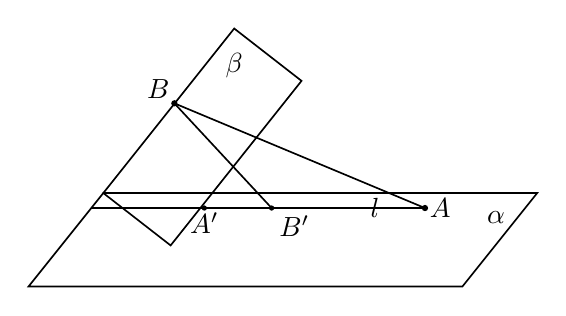
\begin{tikzpicture}[scale=0.95, semithick, every node/.style={inner sep=1.5pt}]
  % 平面 α（水平菱形）
  \draw (-1.2,-0.9) -- (4.6,-0.9) -- (5.6,0.35) -- (-0.2,0.35) -- cycle;
  \node at (5.05,0.02) {$\alpha$};
  % 平面 β（左侧斜置）
  \draw (-0.2,0.35) -- (1.55,2.55) -- (2.45,1.85) -- (0.7,-0.35) -- cycle;
  \node at (1.55,2.05) {$\beta$};
  % 交线 l
  \draw[line width=0.9pt] (-0.35,0.15) -- (3.3,0.15) node[right] {$l$};
  % 关键点
  \coordinate (Ap) at (1.15,0.15);   % A'
  \coordinate (Bp) at (2.05,0.15);   % B'
  \coordinate (A) at (4.1,0.15);
  \coordinate (B) at (0.75,1.55);
  \draw (A) -- (Ap);
  \draw (B) -- (Bp);
  \draw (A) -- (B);
  \fill (Ap) circle (1pt); \node[below] at (Ap) {$A'$};
  \fill (Bp) circle (1pt); \node[below right=1pt] at (Bp) {$B'$};
  \fill (A) circle (1.2pt); \node[right] at (A) {$A$};
  \fill (B) circle (1.2pt); \node[above left] at (B) {$B$};
\end{tikzpicture}
\end{center}
\nopagebreak[4]
\Needspace{4\baselineskip}
\textbf{解析}

（1）$BB'=2$ 为 $B$ 到棱 $l$ 的距离，$B$ 到 $\alpha$ 的距离为 $BB'\sin\dfrac{2\pi}3=\sqrt3$。

（2）以 $A'$ 为原点、$l$ 为 $x$ 轴建系，则 $A(0,3,0)$，$B(\sqrt6,-1,\sqrt3)$，$\overrightarrow{AB}=(\sqrt6,-4,\sqrt3)$，$|\overrightarrow{AB}|=5$，故 $l$ 与 $AB$ 所成角为 $\arccos\dfrac{\sqrt6}5$。

\gkanswer{答案：（1）$\sqrt3$；（2）$\arccos\dfrac{\sqrt6}5$。}

\end{answer}
\begin{answer}
\gksolhead{21}{}

\textbf{题目}：

如图，$M(-2,0)$ 和 $N(2,0)$ 是平面上的两点，动点 $P$ 满足：$\left||PM|-|PN|\right|=2$。

（1）求点 $P$ 的轨迹方程；

（2）设 $d$ 为点 $P$ 到直线 $l:x=\dfrac12$ 的距离，若 $|PM|=2|PN|^2$，求 $\dfrac{|PM|}d$ 的值。
\nopagebreak[4]
\begin{center}% 2008 年重庆卷文科第 21 题：M(-2,0)、N(2,0)，动点 P 满足 ||PM|-|PN||=2；
%   直线 l: x=1/2，d 为 P 到 l 的距离。
% 来源 PDF：gaokaomath-src/普通高考/2008/2008重庆文.pdf
% SHA-256：a3f3321148dc97354de71daf028e7718ef3c3d89e634f94291448acc1f55ce08
% 原页：2008重庆文.pdf 第 2 页（A3 三栏）第 2 栏，书页码 432。
% 重绘依据：按原页画 x、y 轴与 M、N 两点，l 为 x=1/2 的竖直线，P 在第一象限，
%   PM、PN 为实线，O 标在原点。
\begin{tikzpicture}[x=1.05cm, y=1.05cm, semithick, every node/.style={inner sep=1.5pt}]
  \draw[->,>=stealth] (-3.2,0) -- (3.4,0) node[right] {$x$};
  \draw[->,>=stealth] (0,-2.2) -- (0,2.4) node[above] {$y$};
  \node[below left] at (0,0) {$O$};

  \coordinate (M) at (-2,0);
  \coordinate (N) at (2,0);
  \coordinate (P) at (1.35,1.6);

  \draw (0.5,-2.1) -- (0.5,2.3) node[above] {$l:x=\dfrac12$};
  \draw (M) -- (P) -- (N);
  \fill (M) circle (1.2pt); \node[below] at (M) {$M(-2,0)$};
  \fill (N) circle (1.2pt); \node[below] at (N) {$N(2,0)$};
  \fill (P) circle (1.2pt); \node[above right=1pt] at (P) {$P$};
\end{tikzpicture}
\end{center}
\nopagebreak[4]
\Needspace{4\baselineskip}
\textbf{解析}

（1）由双曲线定义 $2a=2$、$c=2$，得 $b^2=3$，轨迹为 $x^2-\dfrac{y^2}3=1$。

\Needspace{5\baselineskip}
（2）设 $P(x,y)$，则 $|PM|=2x+1$，$|PN|=2x-1$，由 $|PM|=2|PN|^2$ 得 $2x+1=2(2x-1)^2$，即 $8x^2-10x+1=0$，取 $x=\dfrac{5+\sqrt{17}}8$。此时 $d=x-\dfrac12$，故

\nopagebreak[4]
\[\frac{|PM|}d=\frac{2x+1}{x-\frac12}=1+\sqrt{17}.\]

\gkanswer{答案：（1）$x^2-\dfrac{y^2}3=1$；（2）$1+\sqrt{17}$。}

\end{answer}
\begin{answer}
\gksolhead{22}{}

\textbf{题目}：

设各项均为正数的数列 $\{a_n\}$ 满足 $a_1=2$，$a_n=a_{n+1}^{\frac32}a_{n+2}$（$n\in\mathbf N^*$）。

（1）若 $a_2=\dfrac14$，求 $a_3$，$a_4$，并猜想 $a_{2008}$ 的值（不需证明）；

（2）若 $2\sqrt2\leqslant a_1a_2\cdots a_n<4$ 对 $n\geqslant2$ 恒成立，求 $a_2$ 的值。

\Needspace{4\baselineskip}
\textbf{解析}

（1）由 $a_1=a_2^{\frac32}a_3$ 得 $a_3=16$，由 $a_2=a_3^{\frac32}a_4$ 得 $a_4=\dfrac1{256}$；指数依次为 $1,-2,4,-8,\dots$，即 $a_n=2^{(-2)^{n-1}}$，故 $a_{2008}=2^{-2^{2007}}$。

（2）令 $b_n=\ln a_n$，由递推得 $b_n=\dfrac32b_{n+1}+b_{n+2}$，特征根为 $\dfrac12$、$-2$，故 $b_n=C\left(\dfrac12\right)^n+D(-2)^n$。若 $D\neq0$，则 $a_n$ 与部分积无界振荡，与 $2\sqrt2\leqslant a_1\cdots a_n<4$ 恒成立矛盾，故 $D=0$。由 $b_1=\ln2$ 得 $C=2\ln2$，于是 $b_2=\dfrac{\ln2}2$，$a_2=\sqrt2$。

\gkanswer{答案：（1）$a_3=16$，$a_4=\dfrac1{256}$，$a_{2008}=2^{-2^{2007}}$；（2）$\sqrt2$。}

\end{answer}